\begin{sloppypar}
Náhled dokumentu je realizován v samostatném podoknu Atomu, které si uživatel může v pracovním prostředí Atomu zobrazit
s pomocí příkazu \mintinline{text}{wootom:togglePreview}, klávesové zkratky (ve výchozím nastavení \textsc{Alt~+~J}),
položky \uv{Wootom: Toggle Preview} v kontextovém menu nebo podpoložky \uv{Toggle Preview} položky \uv{Wootom} v hlavním
menu Atomu.
\end{sloppypar}

Po zobrazení podokna náhledu (nejprve se otevře napravo podokna editoru aktuálně otevřeného souboru, uživatel se poté
může podokno přemístit) je aktuálně otevřený soubor rozparsován do AST.

\begin{sloppypar}
Poté co je dokument rozparsován, je vzniklý AST reprezentující obsah WooWoo dokumentu podán metodě
\mintinline{text}{RenderingManager#render}. Tato metoda přijme kořen AST, získá pro něj příslušnou implementaci
\mintinline{text}{Renderer} (viz výpis kódu \ref{zobrazeni-nahledu-renderer}) z registru
\mintinline{text}{RendererRegistry}, zavolá metodu \mintinline{text}{Renderer#render} na tento kořen a její výsledek
vrátí. Metoda \mintinline{text}{Renderer#render} pak může teoreticky s přijmutým vrcholem dělat cokoliv, ale v typickém
případě vrchol stromu nějakým způsobem tranformuje na HTML, na všechny jeho děti opět zavolá
\mintinline{text}{RenderingManager#render} a výsledky (HTML vrcholy) těchto volání přidá jako obsah do svého HTML. Takto
se renderování postupně zanořuje hlouběji a hlouběji až projde celý AST. Pokud je navíc některý z vrcholů, které
\mintinline{text}{RenderingManager#render} zpracovává, jedním z druhů prvků WooWoo dokumentu, které mají variantu,
před hledáním příslušného \mintinline{text}{Renderer} v \mintinline{text}{RendererRegistry} je navíc získána abstraktní
varianta z \mintinline{text}{VariantRegistry}. Pokud abstraktní varianta nebyla nalezena, je použit výchozí
\mintinline{text}{Renderer}.
\end{sloppypar}

\begin{sloppypar}
Takto je z AST získáno HTML reprezentující logickou strukturu WooWoo dokumentu. Toto HTML je následně podáno metodě
\mintinline{text}{HTMLViewModel#render}, která jej zobrazí uživateli v podoknu pro náhled.
\end{sloppypar}

\begin{listing}
    \caption{Interface \mintinline{typescript}{Renderer}}
    \label{zobrazeni-nahledu-renderer}
    \begin{minted}{typescript}
interface Renderer {
    kind?: WooElementKind;
    abstractVariant?: string;

    render<T extends ASTNode>(
        renderingManager: RenderingManager,
        astNode: T,
    ): Node;
}
    \end{minted}
\end{listing}

Na obrázku \ref{zobrazeni-nahledu-pkm-kapitola} je pro ilustraci zobrazen náhled dokumentu s definicí části (zde
konkrétně kapitoly), jejím meta-blokem a následujícím blokem textu (zdroj dokumentu vzatý ze studijního textu BI-PKM).

\begin{figure}\centering
    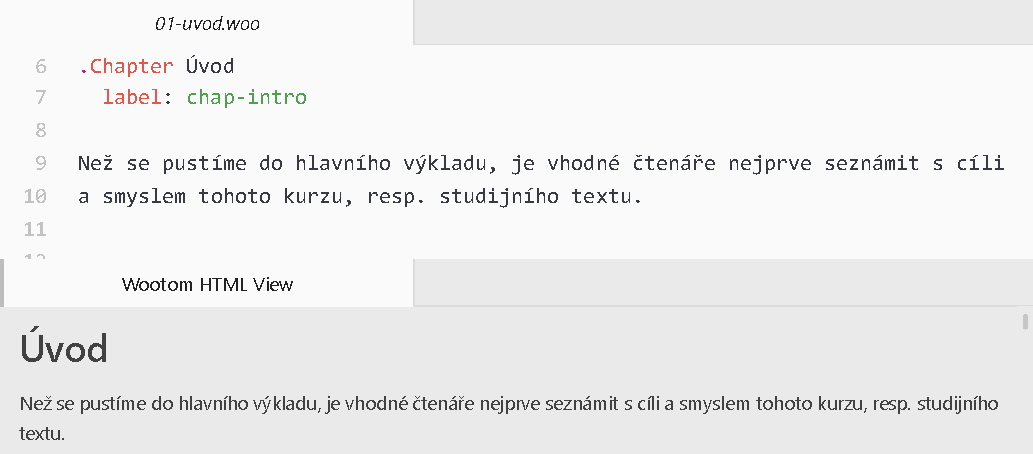
\includegraphics[width=1.0\textwidth]{content/realizace/zobrazení-náhledu-pkm-kapitola}
 	\caption[Náhled části dokumentu]{Náhled části dokumentu ve zdroji studijního textu k BI-PKM~\cite{pkm}}
    \label{zobrazeni-nahledu-pkm-kapitola}
\end{figure}

\begin{sloppypar}
Náhled je živě aktualizován při modifikaci zdrojového souboru. Bylo implementováno jednoduché zobrazování většiny prvků
FIT Template šablony dle stylů existujících výstupů. Zobrazování některých prvků ale zatím podporováno není. Z časových
důvodů nebylo implementováno zobrazení vnějších prostředí \mintinline{text}{.enumerate} a \mintinline{text}{.itemize}
a vnitřního prostředí \mintinline{text}{.item}. Dále nebylo implementováno zobrazování vnějšího prostředí \mintinline
{text}{.image} a vnitřního prostředí \mintinline{text}{.todo}, a to z důvodu jejich absence ve zdrojích existujících
studijních textů. Všechny ostatní prvky jsou (alespoň částečně) zobrazovány.
\end{sloppypar}

Tímto je realizován funkční požadavek \textbf{\ref{F2}} a \textbf{\ref{F3}}. V budoucnu by mohl být náhled vylepšen
například o zobrazení celého dokumentu (nikoliv pouze aktuálně otevřeného souboru) nebo o synchronní posuv náhledu a
zdrojového souboru (což by mělo být možné díky přesným pozicím vrcholů AST).

\subsection{Zobrazování matematických výrazů}

Zobrazování matematických výrazů je na základě provedené rešerše \ref{zobrazovani-matematickych-vyrazu} řešeno za pomoci
knihovny MathJax 2.x s konfigurací SVG výstupu. Uživateli je dále umožněno nadefinovat v nastaveních rozšíření vlastní
makra, která jsou předána konfiguraci knihovny MathJax.

Na obrázku \ref{zobrazeni-nahledu-pkm-matematika} je pro ukázku zobrazen náhled vnitřních matematických prostředí v textu,
jež jsou doplněna o vnější matematické prostředí (blokovou matematiku).

\begin{figure}\centering
    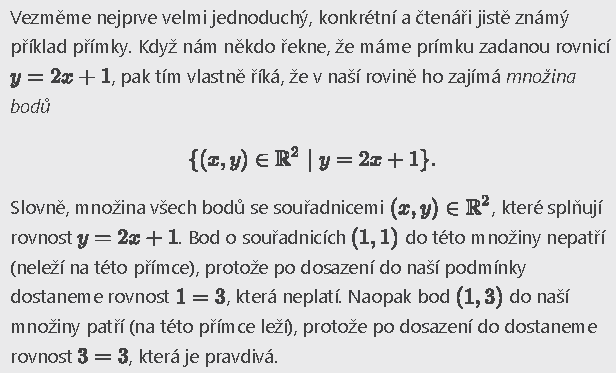
\includegraphics[width=1.0\textwidth]{content/realizace/zobrazení-náhledu-pkm-matematika}
 	\caption[Matematické výrazy v náhledu dokumentu]{Matematické výrazy v náhledu studijního textu k BI-PKM~\cite{pkm}}
    \label{zobrazeni-nahledu-pkm-matematika}
\end{figure}

Protože je sazba matematických výrazů výpočetně náročná, jsou výstupní SVG jsou cachována v paměti (do zavření editoru)
a je-li stejný výraz použit znovu (při obnovení náhledu nebo třeba v jiném souboru), MathJax už volán není a výsledné
SVG je zobrazeno mnohem rychleji (zdánlivě okamžitě).

Byl tak realizován funkční požadavek \textbf{\ref{F4}}.

\subsection{Zobrazování grafických objektů}

Zobrazování TikZ obrázků je na základě provedené rešerše \ref{zobrazovani-grafickych-objektu} řešeno závislostí na
nativní instalaci \TeX{} distribuce. Obdobně jako uživatel může v nastaveních nadefinovat vlastní makra pro MathJax, tak
i zde je umožněno do preambule \LaTeX{} dokumentu, který je použit pro vygenerování obrázku, vložit vlastní obsah (nejen
vlastní makra, ale například i použití dalších \LaTeX{} \textit{packages}).

Při překladu vrcholu AST, který reprezentuje vnější prostředí \mintinline{text}{!tikz}, je nejprve zobrazeno HTML se
(částečně skrytým) zdrojem TikZ. Při tomto překladu je zároveň zavolána asynchronní funkce, která nejprve zkontroluje,
zdali se zdroj obrázku nenachází v cache. Pokud ano, je vrácen obsah cache (kterým je výsledné SVG) a ten je zobrazen
uživateli. Pokud ne, je TikZ zdroj spolu s preambulí (výchozí, nebo uživatelem definovanou) zapsán do dočasného souboru,
na který je zavolán příkaz \mintinline{text}{latex}, jehož výsledkem je DVI soubor (jehož generování je rychlejší, než
PDF). Pro vygenerování SVG z DVI je pak využit příkaz \mintinline{text}{dvisvgm}. Nakonec je SVG výstup přečten, přidán
do cache, jsou uklizeny dočasné soubory a obrázek je zobrazen uživateli. Pokud při procesu nastala chyba, je uživateli
zobrazen namísto obrázku obsah \LaTeX{} logu (log soubor je pak také odstraněn). Cache funguje stejným způsobem jako
cache pro MathJax výstup (je pouze v paměti, po zavření editoru je ztracena).

Protože vygenerované SVG má fixní barvy výplně, je pro podporu různých témat uživatelského rozhraní uživateli umožněno
vybrat v nastaveních jeden ze tří režimů zobrazování těchto SVG výstupů. Výchozím režimem je zobrazení obrázků s bílým
pozadím, dalším režimem pak inverze barev SVG a posledním režimem je zobrazení SVG bez jakýchkoliv změn (není přidáno
pozadí ani pozměněny barvy).

Tímto byl realizován funkční požadavek \textbf{\ref{F5}}. Ukázka náhledu TikZ obrázku se nachází na obrázku \ref
{zobrazeni-nahledu-pkm-tikz}.

\begin{figure}\centering
    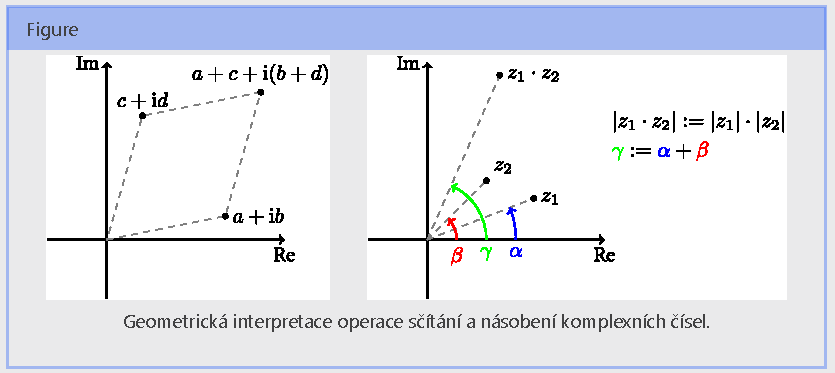
\includegraphics[width=1.0\textwidth]{content/realizace/zobrazení-náhledu-pkm-tikz}
 	\caption[TikZ obrázky v náhledu dokumentu]{TikZ obrázky v náhledu studijního textu k BI-PKM~\cite{pkm}}
    \label{zobrazeni-nahledu-pkm-tikz}
\end{figure}
